\documentclass[italian,12pt]{article} %tipo di documento

%--------------variabili------------------%
\def\Title{Norme di Progetto}
\def\Author{7Last}
\def\Version{v0.2}
%-----------------------------------------%


\usepackage[left=2cm, right=2cm, bottom=3cm, top=3cm]{geometry}
\usepackage{fancyhdr}
\usepackage{graphicx}
\graphicspath{ {../../logo/} }
\usepackage{href-ul}
\usepackage{tikz}
\usepackage{tgadventor}
\usepackage[useregional=numeric,showseconds=true,showzone=false]{datetime2}
\usepackage{caption}
\usepackage{longtable}
\usepackage{xcolor}



% Definizione delle nuove classi di titolo
\titleclass{\subsubsubsection}{straight}[\subsection]
\titleclass{\subsubsubsubsection}{straight}[\subsubsubsection]
\titleclass{\subsubsubsubsubsection}{straight}[\subsubsubsubsection] % nuovo livello

% Creazione dei nuovi contatori
\newcounter{subsubsubsection}[subsubsection]
\newcounter{subsubsubsubsection}[subsubsubsection]
\newcounter{subsubsubsubsubsection}[subsubsubsubsection] % nuovo livello

% Rinnovo dei comandi per la formattazione dei numeri delle sezioni
\renewcommand\thesubsubsubsection{\thesubsubsection.\arabic{subsubsubsection}}
\renewcommand\thesubsubsubsubsection{\thesubsubsubsection.\arabic{subsubsubsubsection}}
\renewcommand\thesubsubsubsubsubsection{\thesubsubsubsubsection.\arabic{subsubsubsubsubsection}} % nuovo livello
\renewcommand\theparagraph{\thesubsubsubsubsubsection.\arabic{paragraph}} % opzionale; utile se i paragrafi devono essere numerati

% Formattazione dei titoli delle sezioni
\titleformat{\subsubsubsection}
  {\normalfont\normalsize\bfseries}{\thesubsubsubsection}{1em}{}
\titleformat{\subsubsubsubsection}
  {\normalfont\normalsize\bfseries}{\thesubsubsubsubsection}{1em}{}
\titleformat{\subsubsubsubsubsection} % nuovo livello
  {\normalfont\normalsize\bfseries}{\thesubsubsubsubsubsection}{1em}{} 

% Spaziatura dei titoli delle sezioni
\titlespacing*{\subsubsubsection}
{0pt}{3.25ex plus 1ex minus .2ex}{1.5ex plus .2ex}
\titlespacing*{\subsubsubsubsection}
{0pt}{3.25ex plus 1ex minus .2ex}{1.5ex plus .2ex}
\titlespacing*{\subsubsubsubsubsection} % nuovo livello
{0pt}{3.25ex plus 1ex minus .2ex}{1.5ex plus .2ex}

\makeatletter
% Rinnovo dei comandi per la formattazione dei paragrafi e sottoparagrafi
\renewcommand\paragraph{\@startsection{paragraph}{6}{\z@}%
  {3.25ex \@plus1ex \@minus.2ex}%
  {-1em}%
  {\normalfont\normalsize\bfseries}}
\renewcommand\subparagraph{\@startsection{subparagraph}{7}{\parindent}%
  {3.25ex \@plus1ex \@minus .2ex}%
  {-1em}%
  {\normalfont\normalsize\bfseries}}

% Definizione dei livelli per il Table of Contents
\def\toclevel@subsubsubsection{4}
\def\toclevel@subsubsubsubsection{5}
\def\toclevel@subsubsubsubsubsection{6} % nuovo livello
\def\toclevel@paragraph{7}
\def\toclevel@subparagraph{8}

% Definizione della formattazione per il Table of Contents
\def\l@subsubsubsection{\@dottedtocline{4}{7em}{4em}}
\def\l@subsubsubsubsection{\@dottedtocline{5}{10em}{5em}}
\def\l@subsubsubsubsubsection{\@dottedtocline{6}{14em}{6em}} % nuovo livello
\def\l@paragraph{\@dottedtocline{7}{18em}{7em}}
\def\l@subparagraph{\@dottedtocline{8}{22em}{8em}}
\makeatother

% Impostazione della profondità dei numeri di sezione e del Table of Contents
\setcounter{secnumdepth}{6} % nuovo livello
\setcounter{tocdepth}{6} % nuovo livello


\linespread{1.2}
\captionsetup[table]{labelformat=empty}
\geometry{headsep=1.5cm}

\renewcommand{\contentsname}{Indice}%imposto il nome dell'indice

\makeindex
\newlistof{tabelle}{tabelle}{Elenco delle tabelle}
\newlistof{immagini}{immagini}{Elenco delle figure}

\renewcommand{\cfttabelletitlefont}{\Large\bfseries}
\renewcommand{\cftimmaginititlefont}{\Large\bfseries}
%-------------------INIZIO DOCUMENTO--------------
\begin{document}

\newgeometry{left=2cm,right=2cm,bottom=2.1cm,top=2.1cm}
\begin{titlepage}
	\vspace*{.5cm}

	\vspace{2cm}
	{
		\centering
		{\bfseries\huge \Title\par}
		\bigbreak
		{\bfseries\Large \Subtitle\par}
		\bigbreak
		{\bfseries\large \Author\par}
		\bigbreak
		{\Date\;-\;\Version\par}
		\vfill

		\begin{center}
			\begin{tikzpicture}
				\clip (0,0) circle (2cm) node {\includegraphics[width=4cm]{logo.jpg}};
			\end{tikzpicture}
		\end{center}
	}

	\vfill

\end{titlepage}

\restoregeometry






















\newpage

\pagestyle{fancy}
\fancyhead{}
\lhead{
	\begin{tikzpicture}
		\clip (0,0) circle (0.5cm);
		\node at (0,0) {\includegraphics[width=1cm]{./../logo/logo.png}};
	\end{tikzpicture}%
}
\chead{\vspace{\fill}\Title\vspace{\fill}}
\rhead{\vspace{\fill}\Version\vspace{\fill}}


%-----------tabella revisioni-----------%
\begin{table}[!h]
    \caption{Versioni}
    \begin{center}
        \begin{tabular}{ l l l l p{9cm} }
            \hline                                                                                 \\[-2ex]
            Ver. & Data       & Autore  & Verificatore            & Descrizione                                   \\
            \\[-2ex] \hline \\[-1.5ex]
                                  \\
            0.1  & 28/03/2024 & Matteo Tiozzo  &    & Inizio scrittura documento                    \\
            0.0  & 28/03/2024 & Matteo Tiozzo &	   & Stesura struttura del documento                           \\
            \\[-1.5ex] \hline
        \end{tabular}
    \end{center}
\end{table}
%---------------------------------------%

\newpage

\tableofcontents

\newpage

\listoftabelle

\newpage

\listofimmagini

\newpage

\section{Introduzione}
\setcounter{subsection}{0}
\subsection{Scopo del documento}
Questo documento ha l’obiettivo di delineare la pianificazione e la gestione delle attività necessarie per la realizzazione del progetto.Vengono approfonditi aspetti chiave come l’\textit{Analisi dei Rischi}, il \textit{modello di sviluppo adottato}, la \textit{pianificazione delle attività}, la \textit{suddivisione dei ruoli}, nonché \textit{stime dei costi} e delle \textit{risorse necessarie}.

\subsection{Scopo del prodotto}
Lo scopo principale del prodotto é quello di permettere all’azienda \textit{Sync Lab S.r.l.} di poter valutare se é conveniente investire tempo e risorse per implementare il capitolato \textit{SyncCity - A smart city monitoring platform}. Una soluzione che, tramite l'uso di dispositivi IoT, permette di monitorare costantemente le città. SyncCity infatti servirà a monitorare e raccogliere dati da sensori posti in città, per poi analizzarli e fornire informazioni utili per la gestione della città stessa. Il prodotto finale sarà un prototipo funzionante che permetterà di visualizzare i dati raccolti in una dashboard.

\subsection{Glossario}
Al fine di evitare ambiguità o incomprensioni riguardanti i termini utilizzati nel documento, verrà adottato un glossario in cui saranno presenti le varie definizioni. La presenza di un termine all'interno del glossario verrà indicata applicando questo particolare \textcolor{red}{\uline{\textit{stile}}}.
\subsection{Riferimenti}
    \subsubsection{Normativi}SONO COMPLETAMENTE BUTTATI A CASO
        \begin{itemize}
            \item \textbf{ISO/IEC 12207:2008} - Systems and software engineering - Software life cycle processes
            \item \textbf{ISO/IEC 31000:2009} - Risk management - Principles and guidelines
        \end{itemize}
    \subsubsection{Informativi}
        \begin{itemize}
            \item T2 - Processi di ciclo di vita del software\\ https://www.math.unipd.it/~tullio/IS-1/2023/Dispense/T2.pdf
            \item T4 - Gestione di progetto\\ https://www.math.unipd.it/~tullio/IS-1/2023/Dispense/T4.pdf
            \item Glossario\\ Link al nostro glossario
        \end{itemize}
\subsection{Preventivo iniziale}
Il preventivo iniziale presentato in fase di candidatura è reperibile al seguente \uline{\href{https://github.com/7Last/docs/blob/main/1_candidatura/preventivo_costi_assunzione_impegni_v2.0.pdf}{link}}. All'interno di tale documento viene calcolato il preventivo iniziale del progetto, che equivale a €12.670,00. In aggiunta viene specificato che il gruppo \textit{7Last} stima di terminare il prodotto entro e non oltre la data 24 Settembre 2024.

\section{Analisi dei rischi}
Durante l'avanzamento del progetto è di fondamentale importanza mitigare gli impatti delle difficoltà riscontrate attraverso una corretta \textit{analisi dei rischi}. È stata inclusa questa sezione in questo documento al fine di evitare che eventuali problematiche possano compromettere il corretto svolgimento del progetto. 
Dopo aver elencato i rischi, vengono identificati una serie di passi da intraprendere nel caso in cui uno di essi si verifichi. Secondo lo standard ISO/IEC 31000:2009 \uline{CAMBIARE IL TIPO DI STANDARD}, il processo di gestione dei rischi si articola in 5 fasi:
\begin{itemize}
    \item \textbf{Identificazione dei rischi}: consiste nel riconoscere le possibili cause di \textcolor{red}{\uline{\textit{rischio}}}, le aree di impatto, gli eventi, le cause e le potenziali conseguenze. Questa fase sarà costituita da un'analisi delle attività che permetteranno di dare vita ad un elenco dei rischi basato sugli eventi che potrebbero influenzare il raggiungimento degli obiettivi. 
    \item \textbf{Analisi dei rischi}: questa fase si compone di un processo di valutazione che contribuisce alla valutazione e alle decisioni sul trattamento dei rischi, identificando le strategie più adeguate.
    \item \textbf{Valutazione dei rischi}: il goal di questa fase è quello di prendere decisioni basati sui risultati dell'analisi dei rischi in modo da poter attuare la migliore strategia di trattamento.
    \item \textbf{Trattamento dei rischi}: dopo l'analisi e la valutazione dei rischi, è di fondamentale importanza decidere come trattare questi rischi, al fine di ridurre il loro effetto. 
    \item \textbf{Monitoraggio e revisione dei rischi}: queste attività richiedono di essere integrate nella pianificazione del del processo di gestione del rischio e richiedono un controllo regolare.
\end{itemize}
I fattori fondamentali per identificare i rischi sono:
\begin{itemize}
    \item Tipologia: rappresenta la categoria di rischio, che può essere organizzativa, tecnologica o comunicativa.
    \item Indice: è un valore numerico incrementale che identifica univocamente il rischio per ogni Tipologia. Rischio elevato equivale a 3, rischio medio equivale a 2, mentre rischio basso equivale a 1.
\end{itemize}
Per una rappresentazione schematica dei rischi, si è deciso di attuare la seguente convenzione: R[Tipologia][Indice].

\begin{table}[!h]
    \subsection{Rischi organizzativi}
    \centering
    \hbox{RO3 - Inesperienza del team nella pianificazione delle attività}
    \vspace{0.3cm}
	\begin{tabular}{|l|p{10cm}|} 
		\hline
		\textbf{Descrizione} & La pianificazione delle attività in un primo periodo può risultare non ottima, questo è dovuto all'inesperienza del team, dalla mancata conoscenza dei requisiti, dalla sovrastima/sottostima delle risorse/tempo necessari.\\ 
        \hline
        \textbf{Probabilità} & Alta. \\
        \hline
        \textbf{Pericolosità} & Alta. \\
        \hline
        \textbf{Rilevamento} & Monitorazione continua di GitHub e con il \textit{Piano di progetto} \\
        \hline
        \textbf{Piano di contingenza} & In caso di difficoltà o ritardi, il \textit{piano di progetto} viene revisionato per conformare le attività in base al progresso. Se un membro segnala impossibilità nel rispettare una scadenza, al responsabile il compito di assegnare più risorse o, in casi più gravi, spostare la scadenza. \\
		\hline
	\end{tabular}
    \caption{Tabella 1: rischio organizzativo \textit{RO3 - Pianificazione delle attivitià}}
    \addcontentsline{tabelle}{subsection}{Tabella 1: rischio organizzativo \textit{RO3 - Pianificazione delle attivitià}}
\end{table}

\begin{table}[!h]
    \centering
    \hbox{RO2 - Impegni personali o universitari}
    \vspace{0.3cm}
	\begin{tabular}{|l|p{10cm}|} 
		\hline
		\textbf{Descrizione} & Gli impegni personali e/o universitari possono limitare la disponibilità di uno o più membri del gruppo. \\ 
        \hline
        \textbf{Probabilità} & Media. \\
        \hline
        \textbf{Pericolosità} & Alta. \\
        \hline
        \textbf{Rilevamento} & Condividendo i propri impegni e indicando la disponibilità, i membri possono concordare vari periodi della settimana per tenere le riunioni e comprendere lo stato di sviluppo del progetto da parte di ciascun membro. \\
        \hline
        \textbf{Piano di contingenza} & Al responsabile il compito di rivedere la suddivisione dei ruoli e compiti in base agli impegni di ciascun membro. In casi gravi deve spostare alcune scadenze e rivedere la pianificazione, se questa non tiene conto di tali incovenienti. \\
		\hline
	\end{tabular}
    \caption{Tabella 2: rischio organizzativo \textit{RO2 - Impegni personali o universitari}}
    \addcontentsline{tabelle}{subsection}{Tabella 2: rischio organizzativo \textit{RO2 - Impegni personali o universitari}}
\end{table}

\begin{table}[!h]
    \centering
    \hbox{RO3 - Ritardi rispetto ai costi previsti}
    \vspace{0.3cm}
	\begin{tabular}{|l|p{10cm}|} 
		\hline
		\textbf{Descrizione} & La sottostima/sovrastima dei costi delle attività a causa dell'inesperienza del team può causare ritardi, spreco di tempo e risorse.  \\ 
        \hline
        \textbf{Probabilità} & Alta. \\
        \hline
        \textbf{Pericolosità} & Alta. \\
        \hline
        \textbf{Rilevamento} & Attraverso il cruscotto e confronto periodico con il Piano di Progetto, il Responsabile può monitorare lo stato di avanzamento del progetto \\
        \hline
        \textbf{Piano di contingenza} & In caso di cambiamenti non gravi, si cerca di implementare rapidamente quanto è rimasto aperto. Se significativo, si discute con il proponente per trovare un accordo su come affrontare i cambiamenti. \\
		\hline
	\end{tabular}
    \caption{Tabella 3: rischio organizzativo \textit{RO3 - Ritardi rispetto ai costi previsti}}
    \addcontentsline{tabelle}{subsection}{Tabella 3: rischio organizzativo \textit{RO3 - Ritardi rispetto ai costi previsti}}
\end{table}

\begin{table}[!h]
    \centering
    \hbox{RO2 - Scarsa collaborazione da parte di uno o più membri}
    \vspace{0.3cm}
	\begin{tabular}{|l|p{10cm}|} 
		\hline
		\textbf{Descrizione} & La possibilità che uno o più membri del gruppo non collaborino attivamente allo sviluppo del progetto. \\ 
        \hline
        \textbf{Probabilità} & Media. \\
        \hline
        \textbf{Pericolosità} & Alta. \\
        \hline
        \textbf{Rilevamento} & Attraverso un conteggio delle volte in cui il membro non è presente. Alla 5 volta scatta una segnalazione interna al team. \\
        \hline
        \textbf{Piano di contingenza} & All'amministratore il compito di comunicare al diretto interessato la sua situazione e di invitarlo a partecipare attivamente allo sviluppo. In caso di risultato negativo, al responsabile il compito di assegnare più risorse o, in casi più gravi, di posticipare la scandeza. \\
		\hline
	\end{tabular}
    \caption{Tabella 4: rischio organizzativo \textit{RO2 - Scarsa collaborazione da parte di uno o più membri}}
    \addcontentsline{tabelle}{subsection}{Tabella 4: rischio organizzativo \textit{RO2 - Scarsa collaborazione da parte di uno o più membri}}
\end{table}

\begin{table}[!h]
    \subsection{Rischi tecnologici}
    \centering
    \hbox{RT3 - Inesperienza nell'uso delle tecnologie adottate}
    \vspace{0.3cm}
	\begin{tabular}{|l|p{10cm}|} 
		\hline
		\textbf{Descrizione} & Dato il livello di esperienza che il \textcolor{red}{\uline{\textit{capitolato}}} richiede, potrebbe verificarsi la necessità da parte di alcuni membri del gruppo di acquisire le competenze necessarie. Questo causerebbe ritardi sia nella fase di progettazione che nello sviluppo.  \\ 
        \hline
        \textbf{Probabilità} & Alta. \\
        \hline
        \textbf{Pericolosità} & Alta. \\
        \hline
        \textbf{Rilevamento} & Dopo aver compreso le competenze di ciascun membro del team, il responsabile deve assegnare i compiti in modo da non rendere il compito troppo facile, ma nemmeno troppo difficile per ciascun membro.  \\
        \hline
        \textbf{Piano di contingenza} & Qualora i membri del gruppo dovessero riscontrare difficoltà nello svolgimento di un'attività, verranno affiancati da un componente con più esperienza in quell'ambito. \\
		\hline
	\end{tabular}
    \caption{Tabella 5: rischio tecnologico \textit{RT3 - Inesperienza nell'uso delle tecnologie adottate}}
    \addcontentsline{tabelle}{subsection}{Tabella 5: rischio tecnologico \textit{RT3 - Inesperienza nell'uso delle tecnologie adottate}}
\end{table}

\begin{table}[!h]
    \centering
    \hbox{RT2 - Perdita di informazioni}
    \vspace{0.3cm}
	\begin{tabular}{|l|p{10cm}|} 
		\hline
		\textbf{Descrizione} & La perdita di informazioni rappresenta un rischio di impatto importante per il progetto. Questo può accadere in caso di guasti hardware, errori umani o malfunzionamenti dei sistemi utilizzati. \\ 
        \hline
        \textbf{Probabilità} & Media. \\
        \hline
        \textbf{Pericolosità} & Alta. \\
        \hline
        \textbf{Rilevamento} & Attraverso la monitorazione continua dei sistemi utilizzati. \\
        \hline
        \textbf{Piano di contingenza} & In caso perdita di informazioni, è necessario poter reperire quelle di riserva, tramite un backup. \\
		\hline
	\end{tabular}
    \caption{Tabella 6: rischio tecnologico \textit{RT2 - Perdita di informazioni}}
    \addcontentsline{tabelle}{subsection}{Tabella 6: rischio tecnologico \textit{RT2 - Perdita di informazioni}}
\end{table}

\begin{table}[!h]
    \centering
    \hbox{RT3 - Problemi di compatibilità tra le tecnologie utilizzate}
    \vspace{0.3cm}
	\begin{tabular}{|l|p{10cm}|} 
		\hline
		\textbf{Descrizione} & Per lo sviluppo del progetto sarà necessario utilizzare tecnologie diverse tra loro. Il malfunzionamento di queste non dipende dal gruppo e sistemare questi guasti potrebbe richiedere tempo e risorse, quindi influire sulla velocità e sui costi del progetto. \\ 
        \hline
        \textbf{Probabilità} & Alta. \\
        \hline
        \textbf{Pericolosità} & Alta. \\
        \hline
        \textbf{Rilevamento} & Solo al momento dell'utilizzo di queste tecnologie il team potrà scoprire se si verificheranno malfunzionamenti o no.  \\
        \hline
        \textbf{Piano di contingenza} & In caso di malfunzionamenti, al responsaibile di progetto il compito di assegnare la quantità di risorse necessarie per la risoluzione di tali, nel minor tempo possibile. \\
		\hline
	\end{tabular}
    \caption{Tabella 7: rischio tecnologico \textit{RT3 - Problemi di compatibilità tra le tecnologie utilizzate}}
    \addcontentsline{tabelle}{subsection}{Tabella 7: rischio tecnologico \textit{RT3 - Problemi di compatibilità tra le tecnologie utilizzate}}
\end{table}


\begin{table}[!h]
    \subsection{Rischi comunicativi}
    \centering
    \hbox{RC1 - Disaccordi all'interno del gruppo }
    \vspace{0.3cm}
	\begin{tabular}{|l|p{10cm}|} 
		\hline
		\textbf{Descrizione} & Disaccordi interni possono derivare da ideologie e opinioni diverse dei componenti.  \\ 
        \hline
        \textbf{Probabilità} & Bassa \\
        \hline
        \textbf{Pericolosità} & Alta. \\
        \hline
        \textbf{Rilevamento} & Attraverso l'opinione dei membri del gruppo e/o l'osservazione delle dinamiche. \\
        \hline
        \textbf{Piano di contingenza} & In caso di disaccordi, si voterà in modo democratico, l'opzione con maggiori voti verrà attuata. \\
		\hline
	\end{tabular}
    \caption{Tabella 8: rischio comunicativo \textit{RC1 - Disaccordi all'interno del gruppo}}
    \addcontentsline{tabelle}{subsection}{Tabella 8: rischio comunicativo \textit{RC1 - Disaccordi all'interno del gruppo}}
\end{table}

\begin{table}[!h]
    \centering
    \hbox{RC2 - Problemi di comunicazione }
    \vspace{0.3cm}
	\begin{tabular}{|l|p{10cm}|} 
		\hline
		\textbf{Descrizione} & Una comunicazione inefficace può causare ritardi, stress, malessere interno del gruppo.  \\ 
        \hline
        \textbf{Probabilità} & Media. \\
        \hline
        \textbf{Pericolosità} & Alta. \\
        \hline
        \textbf{Rilevamento} & Attraverso sondaggi, feedback e comportamenti da parte dei membri del gruppo durante le riunioni o comunicazioni via messaggio. \\
        \hline
        \textbf{Piano di contingenza} & Al responsabile il compito di promuovere comunicazione attiva, organizzare riunioni regolari, indagare sui motivi del malessere e cercare di risolverli. \\
		\hline
	\end{tabular}
    \caption{Tabella 9: rischio comunicativo \textit{RC2 - Problemi di comunicazione}}
    \addcontentsline{tabelle}{subsection}{Tabella 9: rischio comunicativo \textit{RC2 - Problemi di comunicazione}}
\end{table}


\newpage
\newblock\newpage
\newblock\newpage
\newblock\newpage
\newblock\newpage
\newblock
\section{Pianificazione}
\subsection{Modello adottato}

METTERE MODELLO UNA VOLTA DECISO QUALE ADOTTARE
\subsection{Periodi}

Per ogni periodo si riportano di seguito le seguenti informazioni:
\begin{itemize}
    \item Data di inizio, data di fine prevista, data di fine attuale ed eventuali giorni di ritardo
    \item Pianificazione delle attività da svolgere al suo interno (avanzamento atteso), con tanto di potenziali rischi
    \item Tempo stimato per poter completare tutte le attività previste (preventivo)
    \item Confronto fra il lavoro svolto (avanzamento conseguito) e quello preventivato, con annessa analisi dei costi;
    \item Rischi effettivamente occorsi, valutandone il loro impatto e la loro mitigazione;
    \item Retrospettiva di periodo per capire cosa e come migliorare in futuro e cosa invece mantenere.
\end{itemize}
I periodi vengono suddivisi in 3 grandi insiemi corrispondenti alle revisioni di avanzamento del progetto:
\begin{itemize}
    \item \textbf{RTB}: \textcolor{red}{\uline{\textit{\textbf{R}equirements and \textbf{T}echnology \textbf{B}aseline}}}
    \item \textbf{PB}:  \textbf{P}roduct \textcolor{red}{\uline{\textit{\textbf{B}aseline}}}
    \item \textbf{CA}:  \textcolor{red}{\uline{\textit{\textbf{C}ustomer \textbf{A}cceptance}}}
\end{itemize}

\subsection{Requirements and Technology Baseline}
    \subsubsection{Primo sprint:}
        \begin{itemize}
            \item Inizio: 26/03/2024
            \item FIne: 09/04/2024
            \item Fine attuale:
            \item Giorni di ritardo:
        \end{itemize}
        \subsubsubsection{Pianificazione} 
        Questo periodo nasce con l'aggiudicazione dell'appalto da parte del gruppo, il quale si trova a dover iniziare a pianificare le attività da svolgere, prima tra tutte la risoluzione dei problemi segnalati in fase di candidatura. Fatto questo, si prevede di stendere e definire la struttura di ogni documento necessario e di automatizzare il più possibile. In concomitanza a queste attività si prevede un incontro con l'azienda proponente per iniziare la formazione e l'organizzazione delle attività. Il tutto sarà accompagnato da uno studio individuale delle tecnologie che dovranno essere impiegate.\\ Le attività previste sono le seguenti:
        \begin{itemize}
            \item Definire struttura base del documento \textit{Piano di Progetto} e iniziare ad implementarlo
            \item Definire struttura base del documento \textit{Piano di Qualifica}
            \item Definire struttura base del documento \textit{Glossario}
            \item Definire struttura base del documento \textit{Analisi dei requisiti}
            \item Definire struttura base del documento \textit{Norme di progetto}
            \item Studio individuale delle tecnologie
        \end{itemize}
        \subsubsubsubsection{Rischi attesi}
        I rischi attesi per questo periodo sono:
        \begin{itemize}
            \item RT2 - Inesperienza del team
            \item RO2 - Imprecisione nella pianificazione delle attività
            \item RO2 - Elevati costi delle attività
            \item RC1 - Rischio di conflitti interni 
            \item RC1 - Problemi di comunicazione
        \end{itemize}
        Questo è dovuto al fatto che, essendo l'inizio del progetto, non sappiamo ancora come organizzarci per ottimizzare al meglio il tempo e le risorse. La probabilità che si verifichi uno dei rischi elencati è elevata.
        \subsubsubsection{Preventivo}
        Ruoli coinvolti: Amministratore, Responsabile, Verificatore, Analista, Progettista.

        \begin{table}[!h]
            \centering
            \begin{tabular}{ l c c c c c } 
                \hline
                \textbf{} & \textbf{Amministratore} & \textbf{Responsabile} & \textbf{Verificatore} &\textbf{Analista} & \textbf{Progettista} \\
                \hline 
                Tiozzo      & 0 & 0 & 0 & 0 & 0 \\ 
                Malgarise   & 0 & 0 & 0 & 0 & 0 \\ 
                Ferro       & 0 & 0 & 0 & 0 & 0 \\ 
                Benetazzo   & 0 & 0 & 0 & 0 & 0 \\ 
                Occhinegro  & 0 & 0 & 0 & 0 & 0 \\ 
                Baldo       & 0 & 0 & 0 & 0 & 0 \\ 
                Seganfreddo & 0 & 0 & 0 & 0 & 0 \\
                \hline
            \end{tabular}
            \caption{Tabella 10: preventivo orario per ruolo di ciascun membro del team durante il primo periodo}
            \addcontentsline{tabelle}{subsection}{Tabella 10: preventivo orario per ruolo di ciascun membro del team durante il primo periodo}
        \end{table}

            

        \begin{figure*}
            \centering
            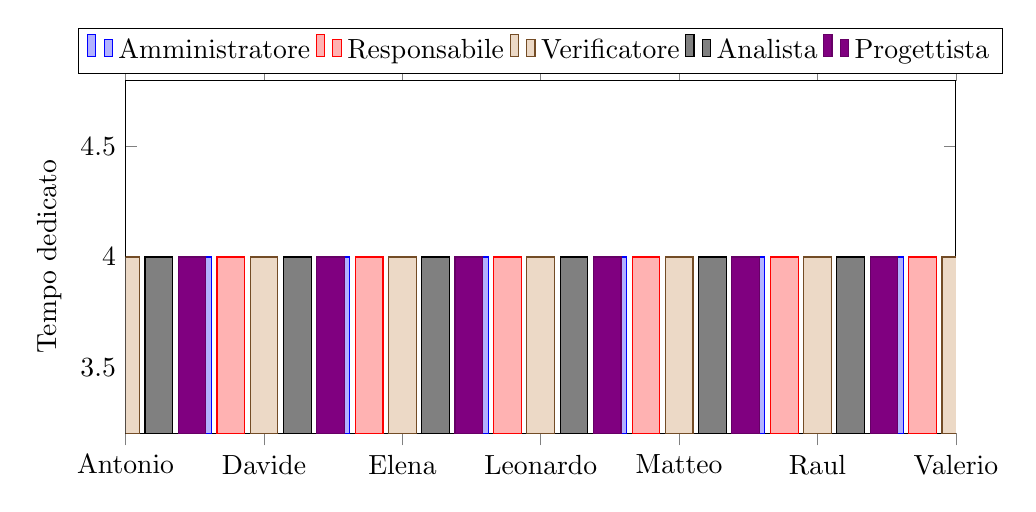
\begin{tikzpicture}
                \begin{axis}[
                    width=\textwidth,
                    height=0.5\textwidth,
                    ybar,
                    enlargelimits=0,
                    legend style={at={(0.5,1.15)},
                      anchor=north,legend columns=-1},
                    ylabel={Tempo dedicato},    
                    symbolic x coords={Antonio, Davide, Elena, Leonardo, Matteo, Raul, Valerio},
                    xtick=data,
                    % nodes near coords,
                    nodes near coords align={vertical},
                    ]
                \addplot coordinates {(Antonio,4) (Davide,4) (Elena,4) (Leonardo,4) (Matteo,4) (Raul,4) (Valerio,4)};
                \addplot coordinates {(Antonio,4) (Davide,4) (Elena,4) (Leonardo,4) (Matteo,4) (Raul,4) (Valerio,4)};
                \addplot coordinates {(Antonio,4) (Davide,4) (Elena,4) (Leonardo,4) (Matteo,4) (Raul,4) (Valerio,4)};
                \addplot coordinates {(Antonio,4) (Davide,4) (Elena,4) (Leonardo,4) (Matteo,4) (Raul,4) (Valerio,4)};
                \addplot coordinates {(Antonio,4) (Davide,4) (Elena,4) (Leonardo,4) (Matteo,4) (Raul,4) (Valerio,4)};
                \legend{Amministratore, Responsabile, Verificatore, Analista, Progettista}
                \end{axis}
            \end{tikzpicture}
        \caption{Figura 1: impegno preventivo per ruolo di ciascun membro del team durante il primo periodo}
        \addcontentsline{immagini}{subsection}{Figura 1: impegno preventivo per ruolo di ciascun membro del team durante il primo periodo}
        \end{figure*}
        
        \begin{figure*}
        \centering
        \begin{tikzpicture}
            \pie[rotate=90, text=legend]{
                20/Verificatore,
                20/Analista,
                20/Amministratore,
                20/Responsabile,
                20/Progettista
            }
        \end{tikzpicture}
        \caption{Figura 2: ripartizione in percentuale dei ruoli nel primo periodo}
        \addcontentsline{immagini}{subsection}{Figura 2: ripartizione in percentuale dei ruoli nel primo periodo}
        \end{figure*}

        \newpage

        \subsubsubsection{Consuntivo}
        Le attività previste sono state tutte svolte con successo. Come si può vedere dal confronto tra preventivo e \textcolor{red}{\uline{\textit{consuntivo}}}:
        \begin{itemize}
            \item Amministratore: 0 ore preventivate, 0 ore effettive
            \item Responsabile: 0 ore preventivate, 0 ore effettive
        \end{itemize}
        \subsubsubsubsection{Prospetto orario}

        \begin{table}[!h]
            \centering
            \begin{tabular}{ l c c c c c } 
                \hline
                \textbf{} & \textbf{Amministratore} & \textbf{Responsabile} & \textbf{Verificatore} &\textbf{Analista} & \textbf{Progettista} \\
                \hline 
                Tiozzo      & 0 & 0 & 0 & 0 & 0 \\ 
                Malgarise   & 0 & 0 & 0 & 0 & 0 \\ 
                Ferro       & 0 & 0 & 0 & 0 & 0 \\ 
                Benetazzo   & 0 & 0 & 0 & 0 & 0 \\ 
                Occhinegro  & 0 & 0 & 0 & 0 & 0 \\ 
                Baldo       & 0 & 0 & 0 & 0 & 0 \\ 
                Seganfreddo & 0 & 0 & 0 & 0 & 0 \\
                \hline
            \end{tabular}
            \caption{Tabella 11: impegno effettivo per ruolo di ciascun membro del team durante il primo periodo}
            \addcontentsline{tabelle}{subsection}{Tabella 11: impegno effettivo per ruolo di ciascun membro del team durante il primo periodo}
        \end{table}
        \newpage
        \subsubsubsubsection{Prospetto economico}

        \begin{table}[!h]
            \centering
            \begin{tabular}{ l c c c c c } 
                \hline
                \textbf{} & \textbf{Ruolo} & \textbf{Ore} & \textbf{Costo} &\textbf{Differenza} \\
                \hline  
                 & Responsabile        & 0 & 0 & 0 \\ 
                 & Amministratore      & 0 & 0 & 0 \\ 
                 & Verificatore        & 0 & 0 & 0 \\ 
                 & Analista            & 0 & 0 & 0 \\ 
                 & Progettista         & 0 & 0 & 0 \\ 
                 & Programmatore       & 0 & 0 & 0 \\ 
                 & Seganfreddo         & 0 & 0 & 0 \\
                Totale preventivo & - & 0 & 0 &0 \\
                Totale consuntivo & - & 0 & 0 & 0\\
                \hline
            \end{tabular}
            \caption{Tabella 12: aggiornamenti economici del progetto al termine del primo periodo, riflettendo le variazioni tra preventivo e ore effettivamente lavorate}
            \addcontentsline{tabelle}{subsection}{Tabella 12: aggiornamenti economici del progetto al termine del primo periodo, riflettendo le variazioni tra preventivo e ore effettivamente lavorate}
        \end{table}
        \subsubsubsubsection{Rischi effettivamente occorsi e loro mitigazione}
        SCRITTURA DEI RISCHI CHE ABBIAMO TROVATO DURANTE QUESTO PRIMO PERIODO E COME LI ABBIAMO RISOLTI
        \subsubsubsection{Retrospettiva}
        SCRITTURA DI COSA ABBIAMO FATTO BENE E COSA ABBIAMO SBAGIATO, COSÌ DA MIGLIORARCI
\newpage
    \subsubsection{Secondo sprint:}
    \begin{itemize}
        \item Inizio: 10/04/2024
        \item FIne: 24/04/2024
        \item Fine attuale:
        \item Giorni di ritardo:
    \end{itemize}
    \subsubsubsection{Pianificazione} 
    SCRIVI QUALCOSA A RIGUARDO (PT. 4.1.1.1 DEGLI OVERTURE)
    \subsubsubsubsection{Rischi attesi}
    I rischi attesi per questo periodo sono:
    \begin{itemize}
        \item Inesperienza del team
        \item Imprecisione nella pianificazione delle attività
        \item Elevati costi delle attività
        \item Rischio di conflitti interni 
        \item problemi di comunicazione
        \item problemi di coordinamento
    \end{itemize}
    Questo perchè, essendo all’inizio del progetto, siamo ancora incerti su molti aspetti di quest’ultimo, ci stiamo attualmente organizzando e dobbiamo apprendere ancora molto, dunque la probabilità di incorrere in qualche problema tra quelli riportati è abbastanza elevata.
    \subsubsubsection{Preventivo}
    Ruoli coinvolti: 
    \subsubsubsection{Consuntivo}
    Le attività previste sono state tutte svolte con successo
    \subsubsubsubsection{Prospetto orario}
    \subsubsubsubsection{Prospetto economico}
    \subsubsubsubsection{Rischi effettivamente occorsi e loro mitigazione}
    \subsubsubsection{Retrospettiva}


    \subsubsection{Terzo sprint:}
    \begin{itemize}
        \item Inizio: 25/04/2024
        \item FIne: 09/05/2024
        \item Fine attuale:
        \item Giorni di ritardo:
    \end{itemize}
    \subsubsubsection{Pianificazione} 
    SCRIVI QUALCOSA A RIGUARDO (PT. 4.1.1.1 DEGLI OVERTURE)
    \subsubsubsubsection{Rischi attesi}
    I rischi attesi per questo periodo sono:
    \begin{itemize}
        \item Inesperienza del team
        \item Imprecisione nella pianificazione delle attività
        \item Elevati costi delle attività
        \item Rischio di conflitti interni 
        \item problemi di comunicazione
        \item problemi di coordinamento
    \end{itemize}
    Questo perchè, essendo all’inizio del progetto, siamo ancora incerti su molti aspetti di quest’ultimo, ci stiamo attualmente organizzando e dobbiamo apprendere ancora molto, dunque la probabilità di incorrere in qualche problema tra quelli riportati è abbastanza elevata.
    \subsubsubsection{Preventivo}
    Ruoli coinvolti: 
    \subsubsubsection{Consuntivo}
    Le attività previste sono state tutte svolte con successo
    \subsubsubsubsection{Prospetto orario}
    \subsubsubsubsection{Prospetto economico}
    \subsubsubsubsection{Rischi effettivamente occorsi e loro mitigazione}
    \subsubsubsection{Retrospettiva}

    \subsubsection{Quarto sprint:}
    \begin{itemize}
        \item Inizio: 10/05/2024
        \item FIne: 24/05/2024
        \item Fine attuale:
        \item Giorni di ritardo:
    \end{itemize}
    \subsubsubsection{Pianificazione} 
    SCRIVI QUALCOSA A RIGUARDO (PT. 4.1.1.1 DEGLI OVERTURE)
    \subsubsubsubsection{Rischi attesi}
    I rischi attesi per questo periodo sono:
    \begin{itemize}
        \item Inesperienza del team
        \item Imprecisione nella pianificazione delle attività
        \item Elevati costi delle attività
        \item Rischio di conflitti interni 
        \item problemi di comunicazione
        \item problemi di coordinamento
    \end{itemize}
    Questo perchè, essendo all’inizio del progetto, siamo ancora incerti su molti aspetti di quest’ultimo, ci stiamo attualmente organizzando e dobbiamo apprendere ancora molto, dunque la probabilità di incorrere in qualche problema tra quelli riportati è abbastanza elevata.
    \subsubsubsection{Preventivo}
    Ruoli coinvolti: 
    \subsubsubsection{Consuntivo}
    Le attività previste sono state tutte svolte con successo
    \subsubsubsubsection{Prospetto orario}
    \subsubsubsubsection{Prospetto economico}
    \subsubsubsubsection{Rischi effettivamente occorsi e loro mitigazione}
    \subsubsubsection{Retrospettiva}

    \subsubsection{Quinto sprint:}
    \begin{itemize}
        \item Inizio: 25/05/2024
        \item FIne: 09/06/2024
        \item Fine attuale:
        \item Giorni di ritardo:
    \end{itemize}
    \subsubsubsection{Pianificazione} 
    SCRIVI QUALCOSA A RIGUARDO (PT. 4.1.1.1 DEGLI OVERTURE)
    \subsubsubsubsection{Rischi attesi}
    I rischi attesi per questo periodo sono:
    \begin{itemize}
        \item Inesperienza del team
        \item Imprecisione nella pianificazione delle attività
        \item Elevati costi delle attività
        \item Rischio di conflitti interni 
        \item problemi di comunicazione
        \item problemi di coordinamento
    \end{itemize}
    Questo perchè, essendo all’inizio del progetto, siamo ancora incerti su molti aspetti di quest’ultimo, ci stiamo attualmente organizzando e dobbiamo apprendere ancora molto, dunque la probabilità di incorrere in qualche problema tra quelli riportati è abbastanza elevata.
    \subsubsubsection{Preventivo}
    Ruoli coinvolti: 
    \subsubsubsection{Consuntivo}
    Le attività previste sono state tutte svolte con successo
    \subsubsubsubsection{Prospetto orario}
    \subsubsubsubsection{Prospetto economico}
    \subsubsubsubsection{Rischi effettivamente occorsi e loro mitigazione}
    \subsubsubsection{Retrospettiva}


    \subsubsection{Sesto sprint:}
    \begin{itemize}
        \item Inizio: 10/06/2024
        \item FIne: 24/06/2024
        \item Fine attuale:
        \item Giorni di ritardo:
    \end{itemize}
    \subsubsubsection{Pianificazione} 
    SCRIVI QUALCOSA A RIGUARDO (PT. 4.1.1.1 DEGLI OVERTURE)
    \subsubsubsubsection{Rischi attesi}
    I rischi attesi per questo periodo sono:
    \begin{itemize}
        \item Inesperienza del team
        \item Imprecisione nella pianificazione delle attività
        \item Elevati costi delle attività
        \item Rischio di conflitti interni 
        \item problemi di comunicazione
        \item problemi di coordinamento
    \end{itemize}
    Questo perchè, essendo all’inizio del progetto, siamo ancora incerti su molti aspetti di quest’ultimo, ci stiamo attualmente organizzando e dobbiamo apprendere ancora molto, dunque la probabilità di incorrere in qualche problema tra quelli riportati è abbastanza elevata.
    \subsubsubsection{Preventivo}
    Ruoli coinvolti: 
    \subsubsubsection{Consuntivo}
    Le attività previste sono state tutte svolte con successo
    \subsubsubsubsection{Prospetto orario}
    \subsubsubsubsection{Prospetto economico}
    \subsubsubsubsection{Rischi effettivamente occorsi e loro mitigazione}
    \subsubsubsection{Retrospettiva}

    \subsubsection{Settimo sprint:}
    \begin{itemize}
        \item Inizio: 25/06/2024
        \item FIne: 09/07/2024
        \item Fine attuale:
        \item Giorni di ritardo:
    \end{itemize}
    \subsubsubsection{Pianificazione} 
    SCRIVI QUALCOSA A RIGUARDO (PT. 4.1.1.1 DEGLI OVERTURE)
    \subsubsubsubsection{Rischi attesi}
    I rischi attesi per questo periodo sono:
    \begin{itemize}
        \item Inesperienza del team
        \item Imprecisione nella pianificazione delle attività
        \item Elevati costi delle attività
        \item Rischio di conflitti interni 
        \item problemi di comunicazione
        \item problemi di coordinamento
    \end{itemize}
    Questo perchè, essendo all’inizio del progetto, siamo ancora incerti su molti aspetti di quest’ultimo, ci stiamo attualmente organizzando e dobbiamo apprendere ancora molto, dunque la probabilità di incorrere in qualche problema tra quelli riportati è abbastanza elevata.
    \subsubsubsection{Preventivo}
    Ruoli coinvolti: 
    \subsubsubsection{Consuntivo}
    Le attività previste sono state tutte svolte con successo
    \subsubsubsubsection{Prospetto orario}
    \subsubsubsubsection{Prospetto economico}
    \subsubsubsubsection{Rischi effettivamente occorsi e loro mitigazione}
    \subsubsubsection{Retrospettiva}

    \subsubsection{Sommario finale}
    \subsubsubsection{Riepilogo prospetto orario}
    \subsubsubsubsection{Ore consumate}
    \subsubsubsubsection{Ore rimanenti}
    \subsubsubsection{Riepilogo prospetto economico}
    \subsubsubsection{Costi totali}

    \subsection{Tra RTB e PB}
    \subsubsection{Ottavo periodo}
    \begin{itemize}
        \item Inizio: 10/07/2024
        \item FIne: 24/07/2024
        \item Fine attuale:
        \item Giorni di ritardo:
    \end{itemize}
    \subsubsubsection{Pianificazione} 
    SCRIVI QUALCOSA A RIGUARDO (PT. 4.1.1.1 DEGLI OVERTURE)
    \subsubsubsubsection{Rischi attesi}
    I rischi attesi per questo periodo sono:
    \begin{itemize}
        \item Inesperienza del team
        \item Imprecisione nella pianificazione delle attività
        \item Elevati costi delle attività
        \item Rischio di conflitti interni 
        \item problemi di comunicazione
        \item problemi di coordinamento
    \end{itemize}
    Questo perchè, essendo all’inizio del progetto, siamo ancora incerti su molti aspetti di quest’ultimo, ci stiamo attualmente organizzando e dobbiamo apprendere ancora molto, dunque la probabilità di incorrere in qualche problema tra quelli riportati è abbastanza elevata.
    \subsubsubsection{Preventivo}
    Ruoli coinvolti: 
    \subsubsubsection{Consuntivo}
    \subsubsubsubsection{Prospetto orario}
    \subsubsubsubsection{Prospetto economico}
    \subsubsubsubsection{Rischi effettivamente occorsi e loro mitigazione}
    \subsubsubsection{Retrospettiva}

% \subsection{Product Baseline}


% \section{Preventivo}
% \subsection{Requirements and Technology Baseline}
%     \subsubsection{Primo sprint:}
%     \subsubsection{Secondo sprint:}
%     \subsubsection{Terzo sprint:}
%     \subsubsection{Quarto sprint:}
%     \subsubsection{Quinto sprint:}
%     \subsubsection{Sesto sprint:}
%     \subsubsection{Settimo sprint:}
% \subsection{Preventivo a finire}
%     \subsubsection{Resoconto finale RTB}
%     \subsubsection{Risuddivisione oraria}

% \section{Consuntivo}
% \subsection{Requirements and Technology Baseline}
%     \subsubsection{Primo sprint:}
%     \subsubsection{Secondo sprint:}
%     \subsubsection{Terzo sprint:}
%     \subsubsection{Quarto sprint:}
%     \subsubsection{Quinto sprint:}
%     \subsubsection{Sesto sprint:}
%     \subsubsection{Settimo sprint:}


\end{document}